\chapter{Background}
\label{sec:background}

Before delving into the nuanced aspects of virtual reality text entry methods, we offer a comprehensive overview by scrutinizing diverse studies and articles. Employing three key questions—``Why is it being implemented,'' ``How is it being executed,'' and ``What is being utilized''—our objective is to underscore the shared intersections and innovative approaches within these studies. Drawing on the Technology Acceptance Model (TAM) as developed by Davis \cite{davis1989}, we apply a theoretical lens to examine these aspects, focusing on the perceived usefulness and ease of use of VR text entry systems. This approach not only helps us understand the factors driving the adoption and practical execution of these methods but also assists in identifying the specific tools and interfaces currently in use. Furthermore, by considering the references and nomenclature utilized, we aim to leverage them as a foundational basis for more advanced research on this subject. This section will conclude by identifying the unexplored areas and the knowledge gaps in the examined studies, offering a structured pathway for future investigations.\\ \\
In the context of \ac{VR}, text entry methods are pivotal for enhancing user interaction and functionality. There are three primary techniques commonly employed: The use of physical devices such as controllers, gamepads, joysticks, and keyboards \cite{dube2019textentry} with or without the pass-through technique, which allows users to see their physical keyboard in the virtual environment. This integration significantly improves typing speed and accuracy \cite{giovannelli2022visual}. 
\begin{figure}[h!]
  \centering
  % First row
  \begin{minipage}{0.48\textwidth}
    \centering
    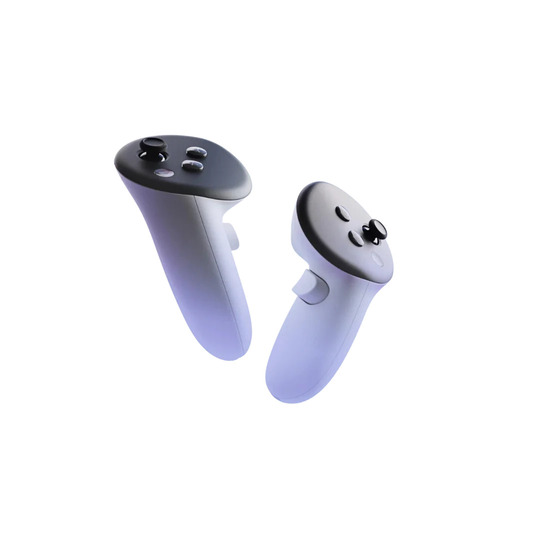
\includegraphics[width=0.35\linewidth]{Background/Quest-3-controllers.png.jpg} % Adjust path and image name
            \captionsetup{justification=centering}

    \caption{VR Controller (\href{https://www.meta.com/de/en/quest/accessories/quest-touch-plus-controller/}{Meta Quest 3})}
  \end{minipage}\hfill
  \begin{minipage}{0.48\textwidth}
    \centering
    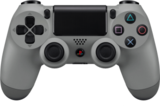
\includegraphics[width=0.4\linewidth]{Background/ps4_controller_png_13_1058.png} % Adjust path and image name
        \captionsetup{justification=centering}

    \caption{ Gamepad (\href{https://www.playstation.com/de-de/accessories/playstation-vr-aim-controller/}{PS Gamepads})}
  \end{minipage}

 
  % Second row
  \begin{minipage}{0.48\textwidth}
    \centering
    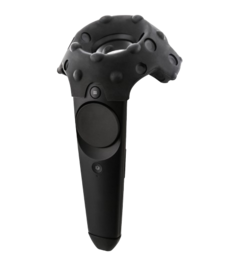
\includegraphics[width=0.3\linewidth]{Background/kisspng-htc-vive-playstation-vr-head-mounted-display-oculu-vive-controller-accessories-5b45845dcff760.0171668615312825258518-removebg-preview.png} % Adjust path and image name
    \caption{Joystick (\href{https://www.vive.com/eu/accessory/controller/}{HTC Vive})}
  \end{minipage}\hfill
  \begin{minipage}{0.48\textwidth}
    \centering
    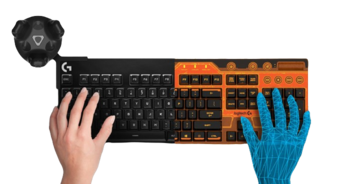
\includegraphics[width=0.48\linewidth]{Background/head-removebg-preview.png} % Adjust path and image name
            \captionsetup{justification=centering}

    \caption{Keyboard (\href{https://www.theverge.com/2017/11/3/16602674/logitech-bridge-sdk-htc-vive-tracker-keyboard}{Logitech})}
  \end{minipage}
\end{figure}
\noindent
Body Gestures, including movements of the head, hands (including fingers), and even blinking, provide alternative interaction methods. For instance, BlinkType and NeckType leverage users’ eye blinks and neck forward and backward movements to select letters , thus offering hands-free interaction\cite{Leng2022}. 

\begin{figure}[h!]
    \centering
    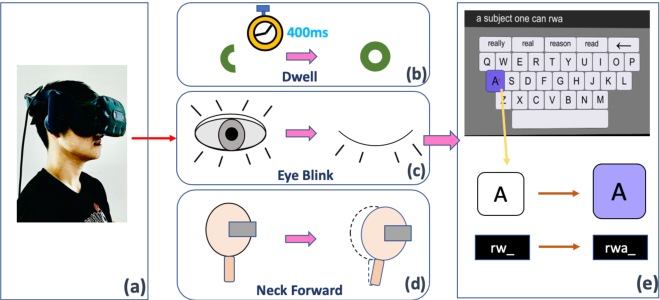
\includegraphics[width=0.7\linewidth]{Background/freehand_Blink.png}
    \caption{An illustration of the text entry with three hands-free techniques in VR \cite{Leng2022}.}
    \label{fig:enter-label}
\end{figure}
\noindent
The realm of haptics also plays a crucial role, with self-referenced haptics focusing on the user's tactile sensations on their own body \cite{hayward2022xr}. Imagine a virtual button placed on the hand of a virtual player; this connection between the user's haptic feedback and their physical presence introduces a new layer of immersion and interaction in \ac{VR} environments.\\ \\ 
Moreover, the Speech-to-Text technique, which converts spoken language into written text, offers a viable alternative when manual entry is impractical or undesired \cite{baljko2006automatic}. The development and refinement of VR text entry techniques have been guided by the need for methods that are both efficient and minimally disruptive, as traditional input devices often do not translate well into \ac{VR} settings \cite{grubert2018text}.\\ \\
The integration of these text entry methods into \ac{VR} applications has opened new avenues for research and development. Studies have shown that the efficiency of text entry systems in\ac{VR} can significantly affect user satisfaction and performance \cite{mcgill2015dovetail}. As \ac{VR} technology continues to evolve, the exploration of more intuitive and natural text entry methods will be crucial. This involves not only technological innovation but also a deep understanding of human-computer interaction principles and user experience design \cite{wickens2015engineering}.\\ \\
Future research should focus on addressing the limitations of current\ac{VR} text entry systems, such as the cognitive load imposed on users and the physical discomfort that may arise from prolonged use. Exploring adaptive systems that can adjust based on the user's input speed and accuracy could provide breakthroughs in usability \cite{hincapie2014metaanalysis}. Additionally, cross-disciplinary studies involving ergonomics, linguistics, and machine learning could lead to the development of more advanced systems that better understand user intent and provide more personalized and context-aware interactions \cite{zhang2017deep}.\\ \\
In conclusion, while significant strides have been made in \ac{VR} text entry technologies, considerable gaps remain in the literature, particularly in terms of comprehensive usability studies and long-term user engagement. Addressing these gaps will not only advance our understanding of \ac{VR} interfaces but also enhance the overall user experience in virtual environments.

\section{Comfortability for virtual typing}
\label{sec:Comfortability for virtual typing} 

In terms of these techniques, long-term comfort is a critical factor when typing on a keyboard within the virtual world. Studies such as those by \cite{dube2019textentry} and \cite{kruger2018text} have highlighted the ergonomic challenges associated with \ac{VR} text entry methods. For instance, head pointing (HP) techniques, where a ray extends from the main camera to facilitate selection, can lead to neck discomfort and dizziness \cite{dudley2019keyboard}. Similarly, Free Hand (FH) and Control Pointing (CP) techniques, while fostering innovation in interaction methods, impose significant physical workloads and can lead to 'gorilla arm fatigue', a term denoting the fatigue resulting from prolonged elevation and use of arms \cite{pseudoHaptics2022}.\\ \\
Moreover, techniques such as Discrete Cursor (DC) and Continuous Cursor (CC) introduce their challenges; both methods may cause texting thumb pain due to repetitive movement \cite{giovannelli2022visual}. An alternative approach involving thumb-to-finger pinch gestures, which offers high spatiotemporal perception and has been reported to increase user satisfaction compared to traditional \ac{VR} keyboards, was explored in \cite{kruger2018text}. This method exemplifies how nuanced gesture control can mitigate some of the physical discomfort associated with more traditional methods.\\ \\
A collaborative study conducted by researchers from the University of Cambridge and the University of Toronto, in partnership with Meta-Reality Labs \cite{leng2022flower}, explored user experiences with different text entry setups in virtual environments. The study found that typing on a virtual keyboard positioned on a physical table led to higher comfort ratings compared to typing in mid-air with either ten or two fingers, showcasing varied comfort levels dependent on the interface used \cite{dudley2019keyboard}. These findings underscore the importance of adaptive interfaces that can dynamically adjust to the user's ergonomic needs and environmental contexts, potentially through the integration of AI-driven systems that learn from user behavior to optimize interface layout and interaction modalities \cite{xu2023haptic}.\\ \\
In addressing the future of \ac{VR} text entry, it is crucial to consider the integration of multimodal feedback systems that combine tactile, visual, and auditory cues to enhance the overall user experience. Such systems could alleviate some of the cognitive and physical strains identified in current technologies by providing more intuitive and natural interaction paradigms \cite{hayward2022xr}. Additionally, advancing haptic technologies could offer more refined and realistic feedback, further enhancing the sense of presence and reducing the disconnect between user actions and system responses \cite{teather2020flik}.\\ \\
Ultimately, the evolution of text entry in virtual reality is contingent upon a multidisciplinary approach that embraces advances in ergonomics, human-computer interaction, and artificial intelligence. By continually refining these systems, we can move closer to creating \ac{VR} environments that are not only effective in terms of task completion but also in promoting user well-being and satisfaction.
\section{Keyboard’s Modernity for virtual typing}
\label{sec: Keyboard’s Modernity for virtual typing} 
Secondly, the modernity of the keyboard in virtual environments is a crucial factor for long-term use. During the study \cite{kruger2018text}, researchers assessed the position and size of the virtual keyboard as essential determinants of usability, emphasizing the keyboard's spatial orientation, including considerations such as left or right-side placement and the optimal distance from the user. The Free Hand (FH) method was noted for its novelty, whereas the Control Pointing (CP) method was found to be most attractive, followed by FH \cite{mcgill2015dovetail}. \\ \\
The type of keyboard consistently used across these studies was Qwerty. However, the shape of the keyboard also impacts usability; two or three-dimensional configurations depend on the application's requirements. For instance, in the study \cite{dudley2019keyboard}, a 2D keyboard was selected because it was fixed to a wooden table and featured keys in a quadratic form, or involved a specific gesture like thumb-to-finger pinch \cite{kruger2018text}. Conversely, another study \cite{pseudoHaptics2022} preferred a 3D keyboard because it floats within the virtual environment, offering a more immersive experience \cite{zhang2017deep}.\\\\
Moreover, the study \cite{teather2020flik} introduced an innovative design called FLIK, where the keyboard keys are arranged in the form of a sphere, deviating from the traditional layout. This spherical arrangement potentially enhances the ergonomic comfort and reduces the cognitive load by aligning more naturally with human hand movements \cite{stanney2019handbook}. Additionally, another study \cite{leng2022flower} pushed the boundaries even further by transforming the keyboard into a flower-shaped configuration while maintaining the order of the QWERTY keys, aiming to combine aesthetic appeal with functional ergonomics \cite{wickens2015engineering}. \\ \\
Each of these innovations reflects ongoing efforts to optimize text entry in virtual environments, highlighting the importance of adaptable interfaces that cater to diverse user needs and preferences \cite{baljko2006automatic, hincapie2014metaanalysis}. As virtual reality technology continues to evolve, the exploration of alternative keyboard layouts and their impacts on user performance and satisfaction will remain a vital area of research \cite{shneiderman2010designing, norman2013design}. \\ \\
The continuous advancement in \ac{VR} technology requires a reevaluation of traditional design principles to include virtual ergonomics and the physiological effects on users, advocating for designs that prevent fatigue and increase user satisfaction \cite{charness2005aging, jacko2009human}.


\section{Keyboard’s Accuracy for virtual typing}
\label{sec: Keyboard’s Accuracy for virtual typing}
When it comes to accuracy, the initial metrics that come into play before pressing a key on the virtual keyboard are key detection and the prevention of typing errors. In a pivotal study \cite{pseudoHaptics2022}, characters are registered when the finger reaches specific distances, precisely 3 cm away from the center of the key (4.5 cm for the Pinch keyboard, as the radius of a sphere was 1.5 cm), and the virtual hands were made semi-transparent to strategically avoid potential collisions. This study proposes a novel technique involving the use of finger-to-thumb as a double-factor confirmation for character entry, enhancing accuracy by confirming intent before final character selection.  \\ \\
Furthermore, the virtual keyboard automatically deactivates all other keys when a collision occurs between the target key and the cursor of the index finger, positioned at the index fingertips to enhance precision during the entry process. This approach is rooted in findings from ergonomic research which suggests that minimizing extraneous movements and providing tactile feedback can significantly reduce entry errors and increase typing speed \cite{mcneill2009gesture, wigdor2011brave}. \\ \\
The integration of spatial and gestural controls as seen in this study aligns with the principles outlined in \cite{norman2013design}, which advocate for natural user interfaces that conform to human motor capabilities and cognitive functions. Additionally, studies such as \cite{zhang2017deep} and \cite{baljko2006automatic} highlight how leveraging deep learning for predictive text input and error correction algorithms can further refine the accuracy of virtual keyboards by anticipating user input and adjusting the interface dynamically. \\ \\
The use of semi-transparent virtual hands and strategic cursor placement also draws upon principles from visual perception psychology, as discussed in \cite{ware2012information}, to reduce visual clutter and enhance the user's focus on target elements, thereby reducing cognitive load and potential input errors. This multidisciplinary approach to interface design, combining HCI, ergonomics, and psychology, is pivotal in developing more intuitive and user-friendly virtual environments \cite{jacko2009human, charness2005aging}.

\section{Haptic Feedback and Visual Feedback in Virtual Environment}

In the realm of feedback within virtual environments, three distinct types are typically identified: haptic, visual, and auditory. In specific studies \cite{teather2020flik, kruger2018text}, haptic feedback primarily involves vibrotactile sensations generated through controllers. This modality not only aids in conveying spatial relationships more effectively than visual and audio feedback alone but also enhances the user’s sense of presence by simulating physical interactions, making these relationships more tangible \cite{hayward2022xr}. \\ \\
While haptic feedback plays a crucial role, visual feedback is also emphasized due to the limited options available for haptic enhancements. In a novel approach, a pseudo-haptic keyboard is introduced with three key features: Protrusion, Hit Effect, and Penetration Blocking \cite{pseudoHaptics2022}. Additionally, a unique pinch keyboard design with bubble-shaped keys is implemented to further enhance user guidance, where the nearest key to the target key is highlighted with a distinct color. Participants in these studies expressed a preference for the Pseudo-haptic and Pinch keyboards, reporting stronger haptic sensation and embodiment compared to a Normal keyboard \cite{zhang2017deep}.\\ \\
Furthermore, another study \cite{teather2020flik} employed a technique called “Big Key,” an algorithm that dynamically adjusts virtual keyboard key sizes based on the likelihood of the next letter in a word. After the initial keystroke, BigKey searches for possible words and scales key sizes according to the frequency of subsequent characters. This approach demonstrated superior performance and high user satisfaction \cite{mcgill2015dovetail}. Conversely, Word Disambiguation, another visual aid technique used in the same study, suggests likely words based on their frequencies as keys are entered, presenting the top three ranked options for efficient word completion. However, this method led to increased frustration and higher mental demand among users \cite{baljko2006automatic}.\\ \\
Each of these feedback mechanisms, whether haptic or visual, plays a pivotal role in shaping the usability and user experience within virtual environments. The integration of advanced feedback techniques, guided by ergonomic and cognitive principles, is crucial for developing interfaces that are both intuitive and effective \cite{jacko2009human, norman2013design}.

\section{Performance for Virtual Typing }
\label{sec: Performance for Virtual Typing}

The performance of virtual typing is not a standalone factor; it is intricately linked to various elements, including the technique employed, the type of feedback (haptic or visual), and the specific use case. Commonly used metrics to measure this performance include Words Per Minute (WPM), Error Rate (ER), Depth of Pressing, Press Duration, and Hand Movements.
Words Per Minute (WPM) is typically defined as the average number of words entered by a user in one minute, with a word usually considered as five characters, including spaces and punctuation:
\begin{equation}
    \text{WPM} = \left( \frac{|T| - 1}{5s} \right) \times 60
  \end{equation} \\ \\
The Error Rate (ER) is the percentage of characters entered incorrectly by the user. ER is calculated by dividing the number of errors by the total number of characters in the text, where \( P \) and \( T \) denote the presented and transcribed text, and MSD is calculated using Levenshtein’s algorithm \cite{levenshteinWiki}:
\begin{equation}
   \text{ER(\%)} = \frac{100 \times MSD(p, T)}{\max(|p|, |T|) }
  \end{equation} \\ \\
Press Duration is the average time that the user's fingers stay on a key after pressing it on the virtual keyboard. This metric can significantly affect the user's feedback, confidence, and satisfaction with \ac{VR} \cite{dube2019textentry}. Additionally, the Depth of Pressing is the average distance that the user's fingers travel in the depth dimension when pressing a key on the virtual keyboard. Depth of pressing can influence the user's fatigue, comfort, and immersion in \ac{VR} \cite{dube2019textentry}.\\ \\
These metrics have been determined through two distinct methods: one involves analyzing the logs generated from keyboard typing, while the other employs a third-party service for calculation. For example, the system in one study \cite{teather2020flik} records the raw input stream. Upon completion, the testbed logs relevant details in a file. In another study \cite{pseudoHaptics2022}, all text entries were conducted through a third-party web application.
\section{Unveiling Omissions}
\label{sec: Unveiling Omissions}

\subsection{Immersion and Realism} 
\label{sec: Immersion and Realism}
Initial studies in the field of \ac{VR} often focused narrowly on haptic feedback limited primarily to simple vibrations, which primarily affected the hand without offering a full spectrum of tactile sensations. This limited approach often led to incomplete sensory experiences, underscoring the need for a more comprehensive exploration of tactile feedback in \ac{VR}. Recent advancements have emphasized the importance of simulating nuanced sensations such as those experienced when grasping or releasing objects. For instance, a study \cite{directionalForce2019} discusses the development of a device that enhances directional sensations in \ac{VR} through mechanical force concentrations using motor rotations. This technology significantly improves the realism of physical interactions, thereby elevating the user's sense of presence and immersion \cite{mcneill2009gesture, stanney2019handbook}.\\ \\
Additionally, the study "Accelerating Skill Acquisition of Two-Handed Drumming using Pneumatic Artificial Muscles" \cite{dasPneumatic} exemplifies the use of advanced haptic systems employing pneumatic artificial muscles to enhance the recall of complex patterns, demonstrating the potential of sophisticated haptic feedback to improve learning and performance in \ac{VR} applications.\\ \\
Moreover, while many studies have focused on distinct text entry methods, there is a notable gap in considering the integration of multimodal inputs, which combine hand gestures with voice commands or elements of auditory and tactile feedback. Such integration is crucial for creating more engaging, convincing, and user-friendly \ac{VR} simulations \cite{wickens2015engineering}. The omission of these synergies could restrict the naturalness and intuitiveness of \ac{VR} text input experiences. Recent research has begun to address these limitations by employing technologies like Word Disambiguation algorithms, which assist in text entry by predicting likely word completions \cite{baljko2006automatic}.\\ \\
Furthermore, while significant attention has been paid to the design of virtual keyboards, there remains a lack of focus on enhancing the virtual hand model to improve interaction during typing tasks. Most studies have maintained a static approach to keyboard orientation in virtual environments, neglecting the potential benefits of a dynamic setup that allows users to navigate and interact more freely within their virtual space. This static approach has often overlooked the significance of environmental textures and other sensory details that could enhance the typing experience and overall interaction quality \cite{spence2008multisensory}.\\ \\
The study "How to Get There When You Are There Already? Defining Presence in Virtual Reality and the Importance of Perceived Realism" \cite{presenceVr2021} further explores the critical role of perceived realism in \ac{VR}. It highlights how users inevitably compare virtual objects with their real-world counterparts and assess their congruence, affecting their overall experience and satisfaction with \ac{VR} technologies \cite{milgram1994taxonomy}.
\subsection{Consistency} 
\label{sec: Consistency}

Consistency in haptic feedback, particularly within virtual environments, has traditionally been limited to static haptic effects—haptic signals that do not change during rendering. This static approach often results in a decrease in user engagement because the repetitive and unchanging nature of the effects fails to mimic the dynamic and varied tactile feedback experienced in real-world interactions \cite{hayward2022xr}. Static haptic feedback can quickly become predictable, reducing the sense of immersion and realism that is crucial for effective virtual environments.
\subsubsection{Challenges of Static Haptic Feedback}
Static haptic feedback systems do not account for changes in user actions or environmental factors, which can lead to a disconnection between the user and the virtual experience. For instance, when interacting with different textures or surfaces in a virtual world, static feedback would fail to provide the nuanced differences users would expect in a real-world scenario \cite{mcgill2015dovetail}. This lack of responsiveness can diminish the perceived quality of the \ac{VR} system and could potentially lead to user dissatisfaction.
\subsubsection{Dynamic Haptic Feedback for Enhanced Engagement}
To address these limitations, more recent studies advocate for dynamic haptic feedback, which adjusts the intensity, pattern, and type of feedback based on the user's interactions and the context within the virtual environment \cite{mcneill2009gesture}. For example, varying the feedback when a user touches different virtual objects—such as changing from a smooth to a textured sensation when moving from a glass surface to sandpaper—can significantly enhance the realism and user engagement.
\subsubsection{Implementations and Technological Advancements}
Several implementations of dynamic haptic feedback have been explored in advanced \ac{VR} systems. Technologies such as haptic suits and gloves equipped with fluid-filled bladders or air pockets that adjust based on the virtual environment have been developed to provide more realistic tactile sensations \cite{stanney2019handbook}. For example, the Teslasuit integrates full-body haptic feedback that can simulate different environmental impacts, from the brush of wind to the impact of a virtual ball.\\ \\
Practical applications of dynamic haptic feedback have been particularly noteworthy in fields such as medical training and remote operations, where the feel of different tissues or materials is crucial. A study involving surgical simulations found that trainees who used \ac{VR} platforms with dynamic haptic feedback performed better and reported a higher level of confidence in their skills compared to those training with static feedback systems \cite{zhang2017deep}.\\ \\
The future of haptic feedback in \ac{VR} is likely to involve a greater integration of AI and machine learning technologies to further refine the responsiveness and adaptability of feedback systems. These advancements could lead to personalized haptic experiences, where the system adjusts not only to general user behavior but also to individual preferences and responses, potentially transforming how users interact with virtual environments \cite{wickens2015engineering}.\\ \\
In conclusion, while static haptic feedback has been a staple in early \ac{VR} applications, the shift towards dynamic, responsive feedback systems represents a significant advancement in the field. By increasing the variability and realism of haptic experiences, \ac{VR} systems can achieve higher levels of user satisfaction and engagement, paving the way for more sophisticated and immersive virtual environments.

\subsection{Skill Transfer and User Experience}
\label{sec:Skill Transfer and User Experience}

Prior research in virtual environments has largely focused on gathering performance data and subjective user feedback, yet often overlooked is the importance of descriptive effects in enhancing user experience. These effects, akin to the MIDI system for musical instruments, represent a method of encoding haptic feedback in a signal-independent manner, which involves detailing only the notes and their 'descriptive' attributes. For example, Apple’s AHAP effect files, part of the CoreHaptics framework, utilize a JSON-based language for describing haptic effects \cite{appleCoreHaptics}. This method allows developers to create expressive and varied haptic sensations without needing a direct motor signal, facilitating richer user interaction. \\ \\ 
Moreover, while metrics like entry speed and error rates are commonly assessed, there is a notable gap in the exploration of other performance indicators that could provide a more holistic view of user experiences. These metrics include the learning curve associated with different text entry methods and the adaptability of users to varying techniques over time. These aspects are critical in understanding the long-term effectiveness and user satisfaction with \ac{VR} interfaces. For example, the accuracy of typing, which is crucial for assessing the effectiveness of text entry methods, can be quantified in several ways:

\begin{equation}
\text{Accuracy in words: } \text{Accuracy} = \left(100\% - \frac{\text{Words with errors} \times 100\%}{\text{Total number of Words}}\right)
\end{equation}

\begin{equation}
\text{Accuracy in characters: } \text{Accuracy} = \left(100\% - \frac{\text{Characters with errors} \times 100\%}{\text{Total number of Characters}}\right)
\end{equation}

\begin{equation}
\text{Accuracy in keystrokes: } \text{Accuracy} = \left(100\% - \frac{\text{Incorrect keystrokes} \times 100\%}{\text{Total number of Keystrokes}}\right)
\end{equation}

\subsubsection{Case Studies and Practical Applications}
Examining case studies where these metrics have been applied reveals their utility in enhancing \ac{VR} training simulations, educational tools, and interactive media. For instance, a \ac{VR} surgical training program that utilized adaptive feedback based on user performance metrics showed that trainees achieved significantly higher accuracy and reduced error rates \cite{vrSurgicalTraining2023}.\\ \\
Another example includes a \ac{VR} language learning application that measured the adaptability of users to different instructional techniques over time, providing valuable insights into how \ac{VR} can be optimized for faster learning curves and better retention rates \cite{vrLanguageLearning2021}.\\ \\
Looking ahead, integrating a broader array of performance metrics into \ac{VR} studies will enhance our understanding and development of user-centric \ac{VR} systems. Future research should also consider the potential of emerging technologies such as artificial intelligence and machine learning to dynamically adapt VR environments to user behaviors, thereby improving the personalization and effectiveness of virtual training environments \cite{aiInVr2023}.\\ \\
In conclusion, while significant strides have been made in capturing performance and subjective data in \ac{VR}, a comprehensive approach that includes descriptive effects and a wider range of performance metrics is essential for the next generation of \ac{VR} applications. Such an approach will not only refine current systems but also pave the way for more sophisticated and immersive user experiences.

\section{Summary}
\label{sec:SummaryBackground}

This chapter provides a comprehensive overview of the varied \ac{VR} text entry methods and their significance in enhancing user interaction and functionality. By employing three key questions—"Why is it being implemented," "How is it being executed," and "What is being utilized"—we have explored the shared intersections and innovative approaches within existing studies. The chapter introduces the primary text entry techniques in \ac{VR}, including the use of physical devices, body gestures, and the Speech-to-Text technique. Each method's role in facilitating effective communication within virtual settings is discussed, highlighting their contributions to reducing cognitive load and increasing typing efficiency.\\ \\
Additionally, the chapter identifies unexplored areas and knowledge gaps in the existing literature, particularly focusing on ergonomic challenges, the integration of adaptive systems, and the need for more comprehensive usability studies. The significance of a multidisciplinary approach involving ergonomics, linguistics, and machine learning is emphasized to foster the development of text entry systems that are both user-friendly and highly functional.\\ \\
In summary, while significant advancements have been made in \ac{VR} text entry technologies, there remains a substantial scope for research, particularly in enhancing the user experience and addressing the limitations of current systems. Future research directions include the exploration of adaptive interfaces and multimodal feedback systems that cater to the ergonomic needs of users and enhance their overall interaction with the virtual environment.

